\documentclass[twocolumn,10pt]{ltjsarticle}

\usepackage[top=20mm,bottom=20mm,left=25mm,right=25mm,columnsep=10mm]{geometry}
\usepackage[haranoaji,nfssonly]{luatexja-preset}
\usepackage{graphicx}
\usepackage{titlesec}
\usepackage{url}

\usepackage{multirow}    % セル結合用
\usepackage{tabularx}    % 表用&カラムサイズ指定

%% カラムサイズの指定用 %%
\newcolumntype{C}[1]{>{\centering\arraybackslash}p{#1}}
\newcolumntype{L}[1]{>{\raggedright\arraybackslash}p{#1}}
\newcolumntype{R}[1]{>{\raggedleft\arraybackslash}p{#1}}

\title{【実験】LombScargleピリオドグラムによるBOS2016の解析2}
\author{山下 尚彦}
\date{\today}

\begin{document}
\maketitle

\section{はじめに}
前回の実験メモで, BOS2016をLomb-Scargleピリオドグラムで解析した結果をまとめたが、
本実験メモでは, 実験の結果から95\%, 99\%, 99.9\%以上周期的であった通信のIPアドレスのペアについてまとめる. 
また, 前回の実験と異なる点がいくつかあるのでそれについても述べたいと思う. 

\section{BOS2016について}
今回の実験で使用するBOS2016は, 総務省実証事業「サイバー攻撃解析・防御モデル実践演習の実証実験の請負」にて実施し, 
研究者コミュニティから提供された組織内ネットワークへの侵害活動を観測されたデータセット\cite{マルウェア対策研42:online}
であり, マルウェア検体のハッシュ値情報や, 通信観測データ, プロセス観測データの他に, Windowsのイベントログや
ファイアウォールのログのデータを保持している. \\
マルウェアの検体は以下の表\ref{tab:bos2016}からわかるように, 動作が確認され通信が発生し, 攻撃の観測ができたものから, 
動作が確認されC2サーバへのSYNパケットのみが送信された検体, C2サーバとの通信を確認できなかったもの, 
検体の実行ができず通信が発生しなかったものがある. 
また, 攻撃活動を観測した検体(表\ref{tab:bos2016}のe04)の通信観測データについてはデータセットに含まれていない.

\begin{table}[htbp]
    \centering
    \caption{BOS2016の検体の挙動と通信について}

    \begin{tabular}{C{2cm}L{1.5cm}L{2.8cm}}
        %% カラム名 %%
        \hline
        観測データ\par ディレクトリ & 挙動 & 通信 \\
        \hline \hline
        %% データ %%
        e04 & 動作 & 攻撃活動を観測 \\ \hline
        e12\par e20 & 動作 & C2サーバとの通信が成立しない(403, 404, 503) \\ \hline
        e43 & 実行不可 & 通信発生せず \\ \hline
        e70\par e435 & 動作 & C2サーバへSYNパケットのみ送信 \\
        \hline
    \end{tabular}
    \label{tab:bos2016}
\end{table}

\section{実験}
\subsection{解析手順}
まず, ネットワーク上の通信を観測したファイル(PCAPファイル)から以下の情報を抽出して,
解析に不要な情報を排除する. 

\begin{itemize}
    \item 通信時間のタイムスタンプ
    \item 送信元IPアドレス
    \item 宛先IPアドレス
    \item 通信プロトコル
    \item 通信データ情報
\end{itemize}

次に,送信元IPアドレスと宛先IPアドレスのペアになるように通信データを分け, 
Lomb-Scargleピリオドグラムで周波数解析を行う. 

\subsection{周期性の測定方法}
Lomb-Scargleピリオドグラムによる信号の周期性はピークを用いることで判断することができる. 
これは, 信号が周期性のない正規分布だという過程に基づいて, 
ある値以上のピークを解析結果が示した場合に周期性があると判断される. 
次に送信元IPアドレス毎にグループ化し, さらに送信元IPアドレス内で宛先IPアドレスでグループ化する. ある確率が0.1\%以上, 
こうすることで送信元と宛先のIPアドレスのペア毎に通信を分けることができたので, 
これをつまり99.9\%周期的であるためには, 図のグラフのピークが0.18631798(${=P_{0.1}}$)以上であることを意味する. 
このグラフのピークは0.9993959064009751と, ${P_{0.1}}$を超えているため99.9\%以上周期的であると言える. 

\begin{figure}[htbp]
    \centering
    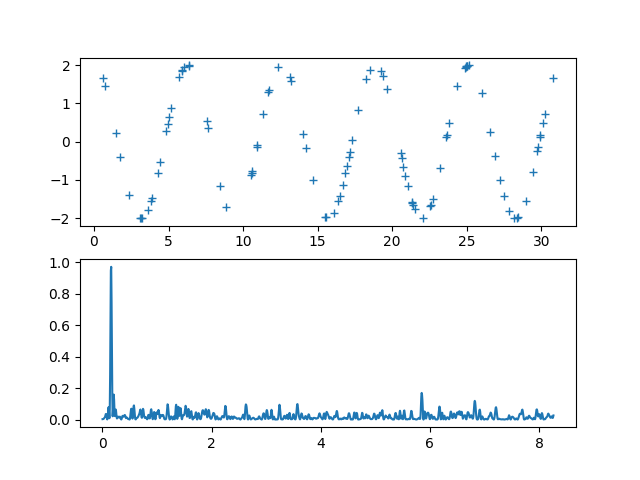
\includegraphics[width=8cm]{images/【実験】LombScargleピリオドグラムによるBOS2016の解析/lombscargle.png}
    \caption{欠損のある正弦波と解析結果}
    \label{fig:lombscargle}
\end{figure}

\subsection{実験データ}
BOS2016のうち, 通信観測データのなかったのe04以外の検体のデータを上記で述べた手順で解析し, 
周期性の測定を行った. 次の章で実験結果について述べる. 

\section{結果}
本章では, 観測データを1日毎に解析した結果と周期性の見られる通信のデータについて述べる. 

以下の表\ref{tab:eXX}から表\ref{tab:e435}は, 観測データを1日ごとに解析し, 
送信IPアドレス数(SRC), 
送信元と宛先IPアドレスのペア数(PAIR), 
通信が周期的でない確率が0.5\%以下のペア数(${P_{0.5}}$), 
通信が周期的でない確率が0.1\%以下のペア数(${P_{0.1}}$), 
通信が周期的でない確率が0.01\%以下のペア数(${P_{0.01}}$)
でまとめた表である.  eXXとeXXXはそれぞれ検体を実行した機器e12, e20, e43, e70とe435の通信を含めた
全体のネットワークを観測したデータである. 

表\ref{tab:e12}, 表\ref{tab:e20}, 表\ref{tab:e43}から, C2サーバと通信が発生しなかった機器(e12, e20, e43)
の通信に周期性はほとんど見られなかったが, 一部で周期的な通信を検出した. 
e12の2016年2月12日に観測された通信で周期的な通信を行ったIPアドレスは10.16.121.16と183.79.197.250のペアである. 
また, e43の2016年2月16日に観測された通信で周期的な通信を行ったIPアドレスは10.16.121.17と23.44.155.27のペアである. 

C2サーバとの通信が発生した機器e70の通信観測データを解析した結果, 表\ref{tab:e70}が示すように
e70の通信に周期性が見られた. 
e70のIPアドレスは10.16.121.19で, 周期性を示した宛先IPアドレスは表\ref{tab:e70_ip}の通りである. 
一方で, e70と同様にC2サーバと通信を行ったe435では周期性のある通信を検出できなかった(表\ref{tab:e435}). 

\begin{table}[htbp]
    \centering
    \caption{eXXの実験結果}

    \begin{tabular}{C{13mm}||L{7mm}L{7mm}L{7mm}L{7mm}L{7mm}L{7mm}}
        %% カラム名 %%
        \hline
        DATE & SRC & PAIR & ${P_{0.5}}$ & ${P_{0.1}}$ & ${P_{0.01}}$ \\
        \hline \hline
        %% データ %%
        20160212  & 168 & 395 & 49 & 37 & 32 \\
        20160213  & 150 & 359 & 51 & 39 & 30 \\
        20160214  & 140 & 330 & 51 & 42 & 34 \\
        20160215  & 150 & 362 & 53 & 40 & 34 \\
        20160216  & 143 & 345 & 61 & 52 & 37 \\
        20160217  & 160 & 382 & 63 & 46 & 29 \\
        20160218  & 136 & 320 & 61 & 47 & 38 \\
        \hline
    \end{tabular}
    \label{tab:eXX}
\end{table}

\begin{table}[htbp]
    \centering
    \caption{eXXXの実験結果}

    \begin{tabular}{C{13mm}||L{7mm}L{7mm}L{7mm}L{7mm}L{7mm}L{7mm}}
        %% カラム名 %%
        \hline
        DATE & SRC & PAIR & ${P_{0.5}}$ & ${P_{0.1}}$ & ${P_{0.01}}$ \\
        \hline \hline
        %% データ %%
        20160328  & 123 & 247 & 47 & 41 & 35 \\
        20160329  & 140 & 315 & 64 & 44 & 36 \\
        20160330  & 149 & 347 & 48 & 38 & 29 \\
        \hline
    \end{tabular}
    \label{tab:eXXX}
\end{table}

\begin{table}[htbp]
    \centering
    \caption{e12の実験結果}

    \begin{tabular}{C{13mm}||L{7mm}L{7mm}L{7mm}L{7mm}L{7mm}L{7mm}}
        %% カラム名 %%
        \hline
        DATE & SRC & PAIR & ${P_{0.5}}$ & ${P_{0.1}}$ & ${P_{0.01}}$ \\
        \hline \hline
        %% データ %%
        20160212  & 21 & 42 & 2 & 0 & 0 \\
        20160213  & 5  & 8  & 0 & 0 & 0 \\
        20160215  & 8  & 14 & 0 & 0 & 0 \\
        20160216  & 4  & 6  & 0 & 0 & 0 \\
        \hline
    \end{tabular}
    \label{tab:e12}
\end{table}

\begin{table}[htbp]
    \centering
    \caption{e20の実験結果}

    \begin{tabular}{C{13mm}||L{7mm}L{7mm}L{7mm}L{7mm}L{7mm}L{7mm}}
        %% カラム名 %%
        \hline
        DATE & SRC & PAIR & ${P_{0.5}}$ & ${P_{0.1}}$ & ${P_{0.01}}$ \\
        \hline \hline
        %% データ %%
        20160215  & 14 & 27 & 0 & 0 & 0 \\
        20160216  & 5  & 8  & 0 & 0 & 0 \\
        20160217  & 5  & 8  & 0 & 0 & 0 \\
        20160218  & 8  & 15 & 0 & 0 & 0 \\
        \hline
    \end{tabular}
    \label{tab:e20}
\end{table}

\begin{table}[htbp]
    \centering
    \caption{e43の実験結果}

    \begin{tabular}{C{13mm}||L{7mm}L{7mm}L{7mm}L{7mm}L{7mm}L{7mm}}
        %% カラム名 %%
        \hline
        DATE & SRC & PAIR & ${P_{0.5}}$ & ${P_{0.1}}$ & ${P_{0.01}}$ \\
        \hline \hline
        %% データ %%
        20160212  & 11 & 20 & 0 & 0 & 0 \\
        20160213  & 8  & 14 & 0 & 0 & 0 \\
        20160216  & 9  & 16 & 2 & 1 & 1 \\
        \hline
    \end{tabular}
    \label{tab:e43}
\end{table}

\begin{table}[htbp]
    \centering
    \caption{e70の実験結果}

    \begin{tabular}{C{13mm}||L{7mm}L{7mm}L{7mm}L{7mm}L{7mm}L{7mm}}
        %% カラム名 %%
        \hline
        DATE & SRC & PAIR & ${P_{0.5}}$ & ${P_{0.1}}$ & ${P_{0.01}}$ \\
        \hline \hline
        %% データ %%
        20160215  & 16 & 34 & 6  & 4  & 3 \\
        20160216  & 7  & 15 & 10 & 10 & 5 \\
        20160217  & 12 & 25 & 6  & 6  & 3 \\
        20160218  & 7  & 16 & 7  & 7  & 6 \\
        \hline
    \end{tabular}
    \label{tab:e70}
\end{table}

\begin{table}[htbp]
    \centering
    \caption{e435の実験結果}

    \begin{tabular}{C{13mm}||L{7mm}L{7mm}L{7mm}L{7mm}L{7mm}L{7mm}}
        %% カラム名 %%
        \hline
        DATE & SRC & PAIR & ${P_{0.5}}$ & ${P_{0.1}}$ & ${P_{0.01}}$ \\
        \hline \hline
        %% データ %%
        20160328  & 16 & 31 & 0 & 0 & 0 \\
        20160329  & 2  & 3  & 0 & 0 & 0 \\
        20160330  & 5  & 9  & 0 & 0 & 0 \\
        \hline
    \end{tabular}
    \label{tab:e435}
\end{table}

\begin{table}[htbp]
    \label{tab:e70_ip}
    \centering
    \caption{e70で周期的な通信を示した宛先IPアドレス}

    \begin{tabular}{|c||c|c|}
        \hline
        DATE & PERIODIC & IP ADDRESS \\
        \hline \hline

        20160215 & ${P_{0.5}}$  & 23.44.155.27 \\ \cline{2-3}
                 & ${P_{0.1}}$  &
                     \begin{tabular}{c}
                        213.165.83.176
                     \end{tabular}\\ \cline{2-3}
                 & ${P_{0.01}}$ &
                     \begin{tabular}{c}
                        10.32.101.160 \\
                        87.106.20.192
                     \end{tabular}\\ \hline

        20160216 & ${P_{0.1}}$  &
                     \begin{tabular}{c}
                        87.106.149.145 \\
                        87.106.20.192
                     \end{tabular}\\ \cline{2-3}
                 & ${P_{0.01}}$ &
                     \begin{tabular}{c}
                        10.32.101.160  \\
                        213.165.83.176 \\
                        50.21.181.152  \\
                        74.208.153.9   \\
                     \end{tabular}\\ \hline

        20160217 & ${P_{0.1}}$  &
                     \begin{tabular}{c}
                        87.106.149.145 \\
                        87.106.253.18
                     \end{tabular}\\ \cline{2-3}
                 & ${P_{0.01}}$ &
                     \begin{tabular}{c}
                        213.165.83.176 \\
                        87.106.20.192
                     \end{tabular}\\ \hline

        20160218 & ${P_{0.1}}$  & 87.106.20.192 \\ \cline{2-3}
                 & ${P_{0.01}}$ &
                     \begin{tabular}{c}
                        213.165.83.176 \\
                        50.21.181.152  \\
                        74.208.153.9   \\
                        87.106.149.145
                     \end{tabular}\\ \hline
    \end{tabular}
\end{table}

\section{考察}
本章では, 前回の実験との比較と実験結果についての考察を行う. 

以下の表\ref{tab:prev_result}は前回の実験結果である. 
前回の実験では, 検体を実行した機器のすべての通信観測データをLomb-Scargleピリオドグラムで解析したが,
今回は通信観測データを分割し, 1日ごとの通信に対して解析を行った. 
そのため, C2サーバとの通信が成立しなかったe12で周期的な通信を検出したり, 逆にC2サーバと通信を行ったe435で
周期的な通信を検出できなかったりと, 前回の実験とは異なる結果を示した. 
e12で異なる結果を示した原因は, 宛先IPアドレス183.79.197.250と通信を行ったのが2016年2月12日の1日のみだったため, 
以前の実験で5日分の観測データに対して解析した際に, 周期性を検出できなかったと考えられる. 
また, e435で周期的な通信を検出できなかったのは, C2サーバとの通信が1日に数回しか発生しておらず, 
1日ごとの観測データでは十分な回数通信していなかったことが要因ではないかと推測される. 

\begin{table}[htbp]
    \centering
    \caption{前回の実験結果}

    \begin{tabular}{C{8mm}L{8mm}L{8mm}L{8mm}L{8mm}L{8mm}L{8mm}}
        %% カラム名 %%
        \hline
        {} & src & pair & ${P_{0.5}}$ & ${P_{0.1}}$ & ${P_{0.01}}$ \\
        \hline \hline
        %% データ %%
        eXX  & 410 & 1183 & 152 & 94 & 65 \\
        e12  & 32  & 63   & 0   & 0  & 0  \\
        e20  & 12  & 23   & 0   & 0  & 0  \\
        e43  & 22  & 42   & 2   & 2  & 1  \\
        e70  & 24  & 49   & 11  & 10 & 6  \\
        eXXX & 217 & 550  & 107 & 73 & 57 \\
        e435 & 20  & 39   & 1   & 1  & 1  \\
        \hline
    \end{tabular}
    \label{tab:prev_result}
\end{table}

\section{おわりに}
本実験メモではLomb-Scargleピリオドグラムを用いてBOS2016を解析し, 周期性の測定を行ったが, 
今回の実験は. 1日ごとに観測データを解析したため前回の実験とは異なる結果がでた. 
その結果, 前回の実験よりも周期性のある通信の検出精度が低下した. 

今後は検出精度の向上とどの程度周期性がある通信を検出するか, また, 通信の内容から
対処の優先度を決定する方法を模索したいと思う. 

\bibliographystyle{junsrt}
\bibliography{DB}
\end{document}